\chapter{Experiments}
\label{ch.experiments}

% Neste capítulo
	This chapter evaluates the performance of communication services of
	the \nanvixmicrokernel running on the \mppa processor, \ie \mailbox
	and \portal. The impacts of the synchronization mechanism were not
	analyzed because it is a simple service that does not directly
	influence node communication, depending greatly on the workload of
	each cluster. Noteworthy, the \sync was used in all benchmarks to
	synchronize the nodes involved due to the different boot times and
	the distinct node roles. The evaluation is divided into two sections.
	First, \autoref{sec.evaluation-methodology} describes the
	micro-benchmarks, their motivations, and the parameters used. Second,
	\autoref{sec.experimental-results} unveil and discusses our
	experimental results.

	\section{Evaluation Methodology}
	\label{sec.evaluation-methodology}

		To deliver a comprehensive assessment of the communication service, we
		stimulate the services with usual collective communication configurations.
		These configurations are usually found in distributed systems and present
		in the high-level services exported by \nanvixmultikernel, such as
		message exchanging between servers and clients, work distribution, and
		gathering results.

        Micro-benchmarks measure the data volume and communication latency
		through the \ioctl interface. In manycores, the nodes that communicate
		with peripherals are the bridge between the user and applications.
		Therefore, in our experiments, \iocluster plays the master role when a
		communication routine requires a master-slave behavior. \ioclusters also
		manages only one of the available interfaces to simplify communication.
		In all micro-benchmarks, only one \pe was used to request microkernel
		services.

		\subsection{Micro-benchmarks}

			To analyze the performance of the communication services, we
			relied in collective communication patters of \mpi, as well as
			common behaviors between clients and servers. The following
			subsections conceptually introduce each of these routines and
			behaviors.

			\subsubsection{Broadcast}

				\textit{Broadcast} is the most widely used communication pattern
				in \mpi. In this routine, a node sends the same data to
				all existing nodes. This process may be implemented in
				several ways, such as, Flat Tree, Binary Tree, Double Tree,
				and Chain~\cite{mpi-survey}. \autoref{fig:exp-broadcast}
				presents the \textit{Flat Tree} algorithm used in the benchmark.
				The Flat Tree defines that the root node should send data
				to everyone without delegating this function to other nodes.
				This routine can be used to send user inputs to a parallel
				program or to send configuration parameters to all
				nodes~\cite{url:mpitutorial}.

				\begin{figure}[!tb]
					\centering%
					\caption{Collective Communication Routines.}%
					\label{fig:mpi-routines}%

					\subcaptionminipage[fig:exp-broadcast]%
						{.35\linewidth}%
						{\mpi Broadcast.}%
						{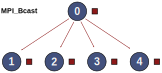
\includegraphics[width=.9\linewidth]{mpi-broadcast.pdf}}%
					\hspace{1cm}%
					\subcaptionminipage[fig:exp-gather]%
						{.35\linewidth}%
						{\mpi Gather}%
						{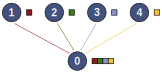
\includegraphics[width=.9\linewidth]{mpi-gather.pdf}}%

					\vspace{0.5cm}%

					\subcaptionminipage[fig:exp-allgather]%
						{.35\linewidth}%
						{\mpi AllGather.}%
						{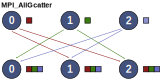
\includegraphics[width=.9\linewidth]{mpi-allgather.pdf}}%
					\hspace{1cm}%
					\subcaptionminipage[fig:exp-ping-pong]%
						{.35\linewidth}%
						{Ping-Pong.}%
						{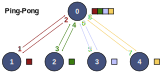
\includegraphics[width=.9\linewidth]{mpi-ping-pong.pdf}}%

					\fonte{Adapted from \citeonline{url:mpitutorial}.}%
				\end{figure}

			\subsubsection{Gather}

				\textit{Gather} is the inverse operation of a broadcast variant
				called scatter. \autoref{fig:exp-gather} illustrates the reverse
				data flow, where this routine gathers the data distributed on a
				single node~\cite{url:mpitutorial}.	Similarly to broadcast, a
				Flat Tree was implemented where all root nodes send their parts
				directly to the root node.

			\subsubsection{AllGather}

				\textit{AllGather} is a routine that does not have a root node,
				illustrated by \autoref{fig:exp-allgather}. As the name suggests,
				the routine performs several Gather operations so that all
				participating nodes end with all pieces of data gathered. Some
				possible algorithms are Ring Algorithm, Recursive Doubling, Gather
				followed by Broadcast Algorithm. The benchmark implements the
				\textit{Bruck Algorithm} where each node will send its data to a
				node with distance $i$ and receive data from a distance $-i$ until
				all nodes contain the complete data.

			\subsubsection{Ping-Pong}

				Ping-Pong is not an \mpi collective communication routine but
				represents communication from a server answering requests from
				client nodes. \autoref{fig:exp-ping-pong} illustrates
				communication by focusing on the master node, where the master
				receives and answers one request at a time.

		\subsection{Experimental Design}
		\label{subsec:experimental-design}

			The parameters that we used for each micro-benchmark are detailed
			in Table~\ref{tab:benchmarks-parameters}.
		% Portal
			The first set of experiments sought to analyze the throughput
			provided by the Portal service. Throughput displays the performance
			of the Portal in communicating different amounts of data and
			thereby highlighting the best amounts. All micro-benchmarks involve
			1 \iocluster and 16 \cclusters, varying the size of the buffer to
			be transmitted from 4~KB to 64~KB. Larger values were not studied
			due to limitation on physical memory size in \cclusters (\ie 2~MB).
			For instance, AllGather requires approximately a total space of
			1~MB ($17$ nodes $\times$ 64~KB).
		% Mailbox
			The second set aimed to analyze the latency of the Mailbox
			service. Latency allows us to analyze the communication time
			between different components of a distributed system. The
			micro-benchmarks executed were practically the same as the
			Portal. However, the buffer size to be transmitted became
			constant, 120~Bytes. The variable parameter of the experiments was
			the number of \cclusters involved in the routines.
			Thus, \iocluster is always the master of routines, and the number
			of \ccluster is changed between 1 and 16.

		% Quantas iterações, limitações de memória e desvio padrão
			The \mppa is designed to provide low energy per operation and time
			predictability which guarantees low variability between runs~\cite{DeDinechin2013-1}.
			Thus, 50 iterations of each benchmark were performed. For each
			experiment, the first ten iterations were discarded to eliminate
			undesired warm-up effects. Finally, all results discussed bellow
			present a standard error inferior to 1\%.

			\begin{table}[!bh]
				\centering%
				\caption{Micro-benchmark parameters for experiments.}%
				\label{tab:benchmarks-parameters}%

				\begin{tabular}{l|c|c|c|l|}
					\cline{2-5}
															 & \multicolumn{2}{c|}{\textbf{Portal}}      & \multicolumn{2}{c|}{\textbf{Mailbox}}    \\ \cline{2-5}
															 & \textbf{\#Clusters} & \textbf{Data Size}  & \textbf{\#Clusters} & \textbf{Data Size} \\ \hline
					\multicolumn{1}{|l|}{\textbf{Broadcast}} & 1 IO, 16 CC         & 4, 8, 16, 32, 64 KB & 1 IO, 1 to 16 CC    & 120 B              \\ \hline
					\multicolumn{1}{|l|}{\textbf{Gather}}    & 1 IO, 16 CC         & 4, 8, 16, 32, 64 KB & 1 IO, 1 to 16 CC    & 120 B              \\ \hline
					\multicolumn{1}{|l|}{\textbf{AllGather}} & 1 IO, 16 CC         & 4, 8, 16, 32, 64 KB & 1 IO, 1 to 16 CC    & 120 B              \\ \hline
					\multicolumn{1}{|l|}{\textbf{Ping-Pong}} & 1 IO, 16 CC         & 4, 8, 16, 32, 64 KB & 1 IO, 1 to 16 CC    & 120 B              \\ \hline
				\end{tabular}

				\fonte{Developed by the author.}%
			\end{table}

	\section{Experimental Results}
	\label{sec.experimental-results}

		In this section, we present our experimental results. First, we
		analyze outcomes for \textit{Portal service}, and next we move to
		a discussion on the results for the \textit{Mailbox service}.

		\subsection{Portal Throughput Analysis}

			\autoref{fig:exp-portal} presents the throughput of the Portal in MB/s
			relative to the different amounts of data transmitted. Results exhibit
			three distinct behaviors in the experiments. First, the Broadcast was
			expected to have the worst transmission rate due to the use of a single
			data transmitter. Since the measurement was done on the receiver side,
			the last slave had to wait for the master to transmit data to all other nodes,
			considerably reducing the transfer rate in the Broadcast. Second, the
			Gather and Ping-Pong routines exhibited similar results, overlapping
			each other on the chart. This similarity is because the master node
			receives multiple requests and handles them serially one by one.
			The master node dictated the data flow in both benchmarks because
			transmission is only performed when allowed by the receiver. Finally,
			the AllGather routine exhibited the best results because of the
			parallelism of communications. Each communication pair is done in parallel
			and multiple read/write requests do not happen at the same time on a node,
			softening the interruption of the master core. In the context of \oss,
			we have subsystems requiring large data transfers, such as file and
			paging systems. In this case, observing the slope of the lines,
			we can infer that the 8~KB and 16~KB sizes favor Portal throughput.
			Overall, the results were as expected, but we believe that solving
			the problem using DMA accelerators described in
			\autoref{sec.mppa-hardware-resources} could significantly improve
			Portal throughput.

			\begin{figure}[!tb]
				\centering%
				\caption{Throughput of the Portal.}%
				\label{fig:exp-portal}%
				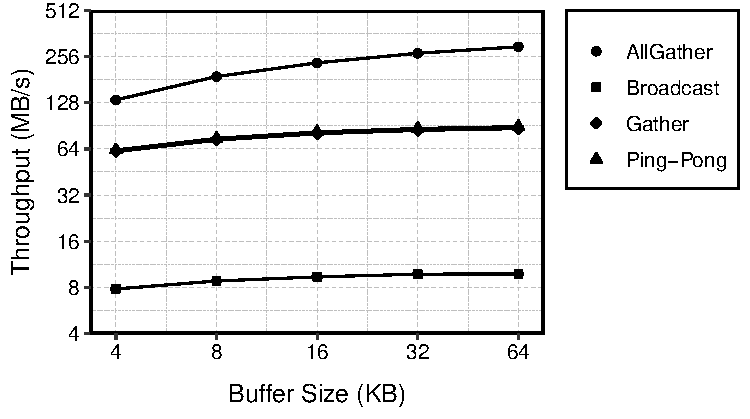
\includegraphics[width=.7\textwidth]{portal-throughput.pdf}%
				\fonte{Develop by the Author.}%
			\end{figure}

		\subsection{Mailbox Latency Analysis}

			\autoref{fig:exp-mailbox} presents the latency of the Mailbox in
			milliseconds relative to the number of clusters involved. First,
			Gather routine, one of the essential routines, had the best results
			because receiving the messages occurs in parallel. Thus, the cost
			after the first message is the overhead of the kernel call itself,
			not the communication. Second, the AllGather routine exhibited similar
			behavior to Gather because sending messages occurs before the reading
			begins. So, when the clusters start reading, the latest messages are
			already coming. The Broadcast routine also suffers from the same problem
			as the Portal routine, because there is only one node sending
			the messages. Finally, the overload of sending
			messages to requesters caused the linear behavior of the Ping-Pong
			routine. In this case, Ping-Pong has a slightly higher cost than the
			sum of Gather and Broadcast costs, because, despite the benefits of
			receiving requests in parallel, the master spends most of its time
			handling requests sequentially. Overall, Broadcast, Gather, and
			AllGather showed how message-passing distributed algorithms can be
			efficiently supported in \nanvixmultikernel. Ping-Pong, in turn,
			highlights the latency of communication between Nanvix subsystems
			with remote kernels, encouraging the potential for improvement using
			\dma accelerators.

			\begin{figure}[!tb]
				\centering%
				\caption{Latency of the Mailbox.}%
				\label{fig:exp-mailbox}%
				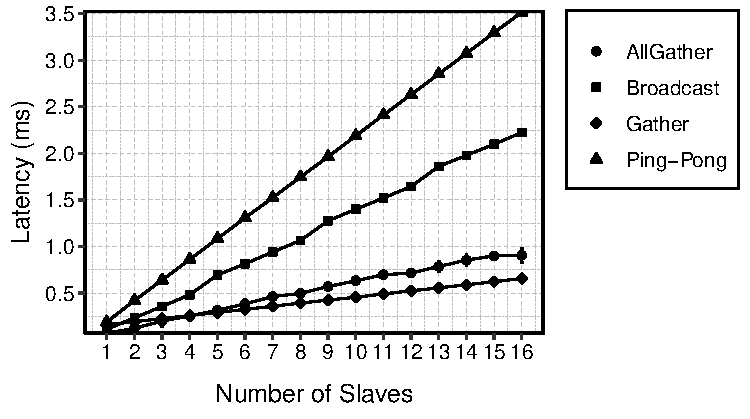
\includegraphics[width=.7\textwidth]{mailbox-latency.pdf}%
				\fonte{Develop by the Author.}%
			\end{figure}
